\subsection{Process analysis}
To get a better understanding of how the application affected the phone it was decided to preform a process analysis.
The process and results are described in this chapter. 

To get a better understanding of how the malicious application affected the overall performance of the phone a process analysis was performed in Android studio.
With the profiler in Android studio it was possible to check the CPU usage, memory usage and network usage.
During the process analysis it became clear that the network and CPU usage stayed at 0\%, however the memory usage kept slowly increasing over time.
The two pictures described below were made at the startup and installation of the malicious applications and after an hour of running the application and showed the memory usage over time.

\begin{figure}[H]
    \centering
    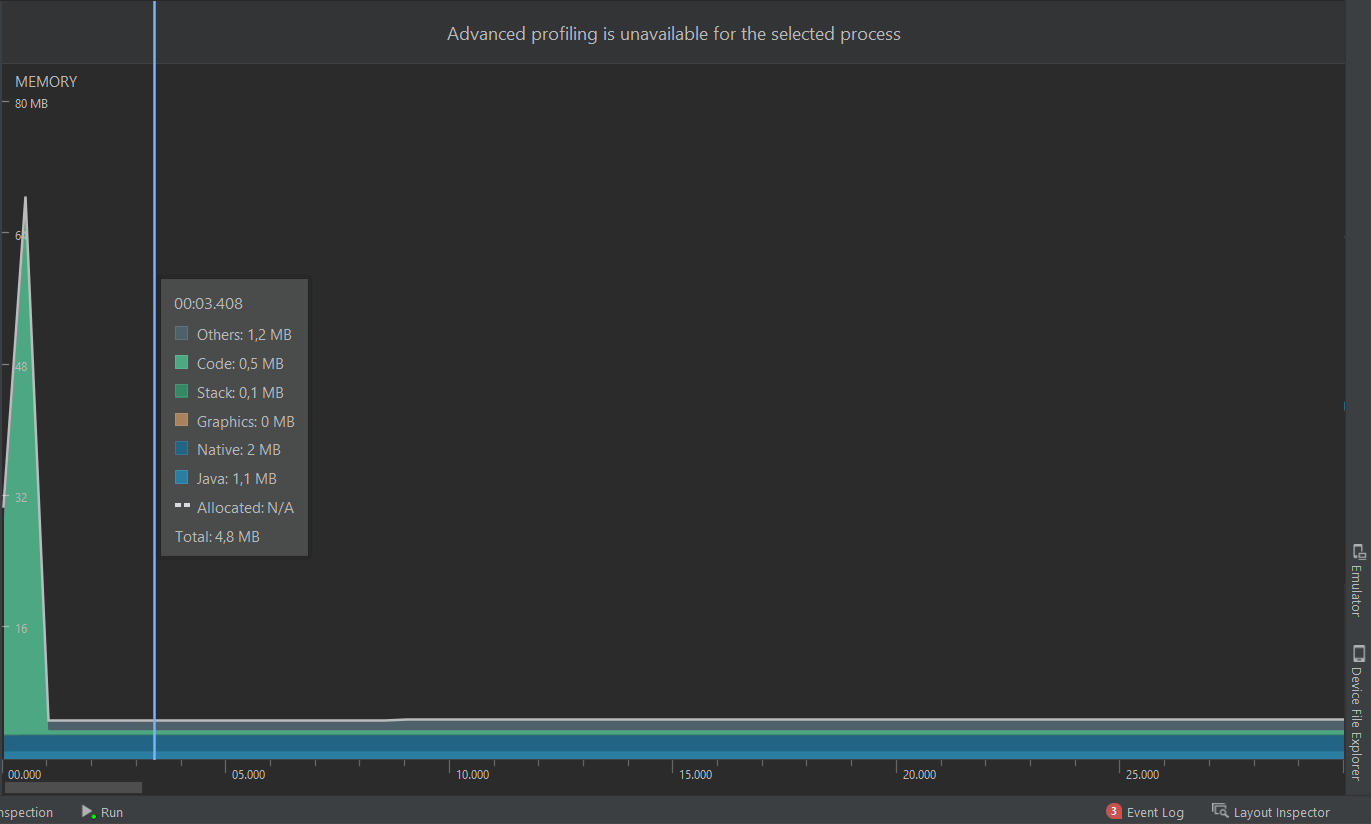
\includegraphics[width=1\textwidth]{MemoryStart.PNG}
    \caption{Memory on startup and installation of the application}
    \label{jordy-memorystartup}
\end{figure}

\begin{figure}[H]
    \centering
    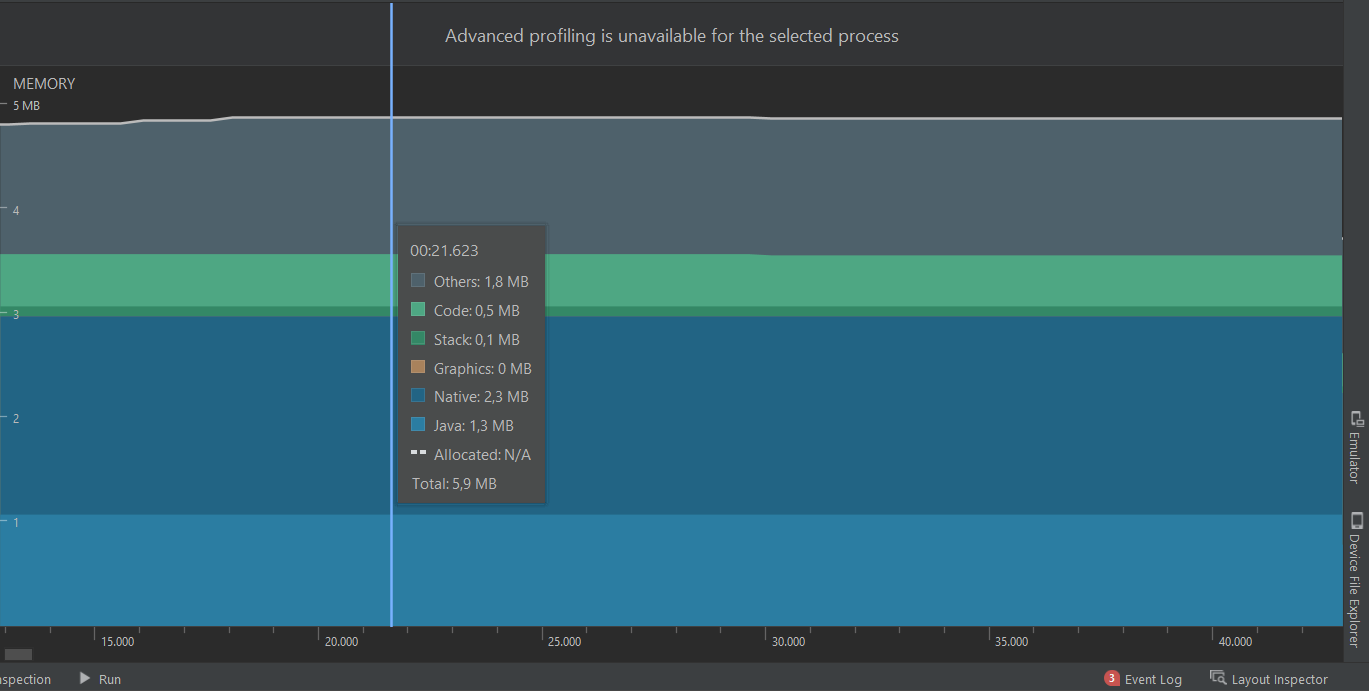
\includegraphics[width=1\textwidth]{MemoryEnd.PNG}
    \caption{Memory after an hour of running the application}
    \label{jordy-memory1hour}
\end{figure}

In the memory usage it was shown that the memory being used very slowly increased.
The areas that the memory usage increased in were the others, native and java areas.
This did not give any more information about why the memory usage slowly increased but it was interesting to see.